\documentclass{article}
\usepackage{babel}
\selectlanguage{english}
\usepackage{amsmath}
\usepackage{amssymb}
\usepackage[colorlinks=true, linkcolor=blue]{hyperref}
\usepackage{xcolor}
\usepackage[top=2cm, bottom=2cm,
            left=1.5cm, right=1.5cm]{geometry}
\usepackage{listings}
\usepackage{url}
\usepackage{graphicx}
\usepackage{cite}

% --- Inline style for code-level names (AthenaK variables, files, flags) ------
\definecolor{varbg}{HTML}{EEF1F7}
\definecolor{varfg}{HTML}{273C75}
\newcommand{\var}[1]{%
  {\setlength{\fboxsep}{1.5pt}%
   \colorbox{varbg}{\textcolor{varfg}{\texttt{\small #1}}}}}

% --- Run-in headers for the individual steps of a workflow -------------------
% Small caps + rule instead of \textbf, so they read as a level below
% \subsubsection rather than as another heading of the same weight.
\definecolor{stepfg}{HTML}{1A6B62}
\newcommand{\step}[1]{%
  \par\medskip\noindent
  {\color{stepfg}\rule[-0.15ex]{2pt}{1.5ex}\hspace{0.5em}\scshape #1}%
  \hspace{0.75em}\ignorespaces}

\begin{document}
\section*{Ejecta and neutrino analysis routines for AthenaK}
\textit{This document summarizes the routines and equations used to compute the
ejecta properties and the neutrino luminosities/average energies from the
spherical-surface output of an AthenaK simulation. Both pipelines share the same
structure: dump a set of fields onto an extraction sphere, process every snapshot
in parallel, and accumulate the per-snapshot results in time.}

\subsection*{Ejecta analysis}
\subsubsection*{Spherical output}
The ejecta analysis operates on data dumped onto AthenaK spheres. One output
block is needed per variable; a block looks as follows:
\begin{verbatim}
<output1>
file_type  = sph
variable   = mhd_w_bcc
dt         = 10.0
radius     = 400.0
ntheta     = 256
\end{verbatim}
Six variables are required at each output time and radius: the primitive MHD
variables (\var{mhd\_w\_bcc}), the ADM three-metric $\gamma_{ij}$ (\var{adm}),
the lapse $\alpha$ (\var{z4c\_alpha}), and the three shift components $\beta^i$
(\var{z4c\_betax}, \var{z4c\_betay}, \var{z4c\_betaz}). AthenaK names the resulting
files \var{<job>.r=<radius>.<variable>.<counter>.vtk}, where \var{<job>} is the job
name of the run; the pipeline reproduces that pattern from its \var{-{}-jobname} and
\var{-{}-radius} arguments. The blocks must therefore all use the same \var{radius},
since the pipeline matches files by the radius string in the file name. Useful radii
are $300.0$ and $400.0$ (code units, $M_\odot$).
Spherical output is storage intensive, so \var{dt} should be chosen as a
compromise: small enough to resolve the ejecta rate in time, large enough to
keep the data volume manageable.

\subsubsection*{Pipeline}
The pipeline is part of KPlot (\url{https://github.com/spacetimecurv/KPlot}), where it
lives in the \var{kplot.sphere} subpackage; it was integrated from
\url{https://github.com/yiqiu0714/AthenaK_BNS_visualization}, in which it formed the
\var{sph\_data\_analysis} scripts. The module \var{kplot.sphere.ejecta} does the bulk
of the work, and is exposed as the console script \var{kplot-sphere-ejecta}. Its
inputs are:
\begin{itemize}
  \item the batchtools (\url{https://github.com/computationalrelativity/batchtools/tree/master})
        segment directories holding the sph output (\var{-{}-sph-dir}, repeated once
        per segment);
  \item the path to the EOS table in \var{.h5} format (\var{-{}-eos-table}), which can
        be produced with PyCompOSE (\url{https://github.com/computationalrelativity/PyCompOSE});
  \item the extraction radius of the spherical output (\var{-{}-radius}) and the
        AthenaK job name prefixing the files (\var{-{}-jobname});
  \item the density floor used in the simulation (\var{-{}-dfloor});
  \item the merger time in geometric units (\var{-{}-t-merger}) together with the
        post-merger window (\var{-{}-t-post-ms}), which set the cutoff time of the
        histograms;
  \item the directory the results are written to (\var{-{}-output-dir}).
\end{itemize}
Every input is a command-line argument, so the module needs no editing; omitted
arguments fall back to the defaults documented by \var{kplot-sphere-ejecta -{}-help}.
The same inputs are available to Python callers through \var{ejecta.analyze()}.

In practice it is easier to drive everything through \var{run\_analysis.sh} in
\var{scripts/sphere/}: it reads the machine-specific paths and the run parameters from
\var{config.ini} next to it, auto-discovers all \var{output-*/sph} segment directories
under \var{simpath}, obtains the merger time from the GW $(2,2)$ mode via
\var{kplot-sphere-mergertime}, and passes everything on as command-line arguments. The
ejecta and neutrino analyses share no state and are run concurrently by the wrapper.
The configuration file is plain INI and is parsed, never executed:
\begin{verbatim}
[paths]
simpath   = /path/to/sim         # parent of the output-XXXX segments
eos_table = /path/to/DD2.h5      # PyCompOSE table, required for the ejecta

[parameters]
jobname   = bhns                 # job name prefixing the sph files
radius    = 400.0                # sph extraction radius   -> --radius
wf_radius = 400                  # GW radius for the merger time
t_post_ms = 15.0                 # post-merger window      -> --t-post-ms
dfloor    = 1e-14                # simulation density floor
n_workers = 8                    # parallel snapshot workers
\end{verbatim}
Only \var{simpath} is mandatory; any parameter left blank is omitted, so the
corresponding module default applies. A copy of the file with all keys documented
ships as \var{config.example.ini}, and the local \var{config.ini} is gitignored so
machine-specific paths never get committed.

\subsubsection*{Workflow}
\step{EOS setup} The script loads the 3D \var{.h5} equation of state and builds
\var{RegularGridInterpolator} objects on the table axes $(\ln n_b, Y_e, \ln T)$,
where $n_b$ is the baryon number density [fm$^{-3}$], $Y_e$ the electron fraction
and $T$ the temperature [MeV]. The two interpolated quantities are the tabulated
CompOSE grids
\begin{align}
  Q_7 &= \frac{e}{n_b m_n}-1,\\
  \frac{Q_1}{m_n} &= \frac{p}{n_b m_n}
\end{align}
i.e.\ the specific internal energy and the pressure normalized by the rest-mass
energy density. Here $e$ is the energy density, $p$ the pressure and $m_n$ the
neutron mass. From the same grids the minimum specific enthalpy over the whole
table is computed,
\begin{align}
  h_{\min}=\min\left(1+Q_7+\frac{Q_1}{m_n}\right)
         =\min\left(\frac{e}{n_b m_n}+\frac{p}{n_b m_n}\right),
\end{align}
which is the reference value for the Bernoulli unbound criterion.

\step{Loading a snapshot} Each of the six sph files of a snapshot is read with
the \var{SphericalData} class of plot-tools
(\url{https://github.com/jfields7/plot-tools}). From \var{mhd\_w\_bcc} we extract
the rest-mass density $\rho$ (\var{dens}), the electron fraction $Y_e$ (\var{s\_00}),
the temperature $T$ (\var{temperature}) and the velocity components
$\tilde{u}^x,\tilde{u}^y,\tilde{u}^z$ (\var{velx}, \var{vely}, \var{velz}), which
are the Valencia-frame spatial four-velocity components. From \var{adm} we extract
the metric components $g_{xx}$, $g_{xy}$, $g_{xz}$, $g_{yy}$, $g_{yz}$, $g_{zz}$, and
from the gauge files the lapse $\alpha$ and the shift $\beta^x,\beta^y,\beta^z$.

The sph output repeats points on the seam and at the pole, so every field is
multiplied by a duplication-correction factor. The factor is determined from the
\var{z4c\_alpha} field: if the values at $\phi=\phi_{\min}$ exceed one, that seam
is duplicated and gets weight $1/2$; if the values at $\theta=\theta_{\min}$ exceed
one, the pole ring is duplicated four times and gets weight $1/4$. Elsewhere the
factor is $1$.

\step{Thermodynamics} The baryon number density is obtained from $\rho$ by a unit
conversion, $n_b=\rho_{\mathrm{cgs}}\cdot 10^{-39}/m_n$ [fm$^{-3}$]. The triples
$(\ln n_b, Y_e, \ln T)$ are clipped to the table bounds and inserted into the two
interpolators, yielding $e_{\mathrm{intp}}\equiv Q_7$ and
$(p/\rho)_{\mathrm{intp}}\equiv Q_1/m_n$ at every surface point. The specific
enthalpy then follows as
\begin{align}
  h = 1 + e_{\mathrm{intp}} + (p/\rho)_{\mathrm{intp}}.
\end{align}

\step{Kinematics} The Lorentz factor is
\begin{align}
  W = \sqrt{1+g_{xx}\tilde{u}_x^2+g_{yy}\tilde{u}_y^2+g_{zz}\tilde{u}_z^2
      +2g_{xy}\tilde{u}_{x}\tilde{u}_{y}+2g_{xz}\tilde{u}_{x}\tilde{u}_{z}
      +2g_{yz}\tilde{u}_{y}\tilde{u}_{z}},
\end{align}
and gives the time component of the four-velocity
\begin{align}
  u^t = \frac{W}{\alpha}.
\end{align}
The spatial four-velocity components in the coordinate frame and their radial
projection are
\begin{align}
  u^x &= \tilde{u}^x-\beta^{x}u^t,\\
  u^y &= \tilde{u}^y-\beta^{y}u^t,\\
  u^z &= \tilde{u}^z-\beta^{z}u^t,\\
  u_r &= u^x\sin{\theta}\cos{\phi}+u^y\sin{\theta}\sin{\phi}+u^z\cos{\theta}.
\end{align}
The covariant time component, which decides whether a fluid element is bound, is
\begin{align}
  u_t =& -\alpha W
        +g_{xx}\beta^{x}\tilde{u}^{x}+g_{yy}\beta^{y}\tilde{u}^{y}+g_{zz}\beta^{z}\tilde{u}^{z}\\
       &+g_{xy}\left(\beta^{x}\tilde{u}^{y}+\beta^{y}\tilde{u}^{x}\right)
        +g_{xz}\left(\beta^{x}\tilde{u}^{z}+\beta^{z}\tilde{u}^{x}\right)
        +g_{yz}\left(\beta^{y}\tilde{u}^{z}+\beta^{z}\tilde{u}^{y}\right).
\end{align}

\step{Masks} A point contributes to the outflow if it lies above the density
floor and moves outwards, $\rho>\rho_{\mathrm{floor}}$ and $u_r>0$. Within that
outflow mask, the unbound points are selected by:
\begin{itemize}
  \item Geodesic criterion: $u_t < -1$
  \item Bernoulli criterion: $hu_t < -h_{\mathrm{min}}$
\end{itemize}

\step{Surface integrand} With the determinant of the three-metric
\begin{align}
  \gamma &= g_{xx}g_{yy}g_{zz}+2g_{xy}g_{xz}g_{yz}-g_{xx}g_{yz}^2-g_{yy}g_{xz}^2-g_{zz}g_{xy}^2,
\end{align}
the base integrand of the mass flux through the sphere reads
\begin{align}
  b = \rho\, u_r \sqrt{\gamma}\,\alpha\, r^2\sin{\theta}.
\end{align}
Multiplying by the per-cell Riemann weights $R_w$ (the products
$\Delta\theta\,\Delta\phi$ from the midpoint rule, with the pole cells divided by
$N_\phi$ so the singular axis is not counted $N_\phi$ times) gives the cell rate
$c_r = b\,R_w$. Applying the geodesic and the Bernoulli mask to $c_r$ defines the
corresponding flux rates $f_r$, and the ejecta rate of each criterion is their sum
over the surface,
\begin{align}
  \dot{M}_{\mathrm{ej}} = \sum f_r .
\end{align}
The velocity at infinity follows from the Lorentz factor with which the fluid element
reaches infinity. Both criteria state that a conserved quantity along the streamline
equals its asymptotic value, so
\begin{align}
  \gamma_{\infty}^{\mathrm{geo}} &= -u_t, &
  \gamma_{\infty}^{\mathrm{Ber}} &= -\frac{hu_t}{h_{\mathrm{min}}},
\end{align}
where the Bernoulli case assumes the enthalpy relaxes to $h_{\mathrm{min}}$ as the
material expands, converting its internal energy into kinetic energy. With
$v_{\infty}=\sqrt{1-\gamma_{\infty}^{-2}}$ this gives
\begin{align}
  v_{\infty}^{\mathrm{geo}} &= \sqrt{1-u_t^{-2}}\quad\text{where } u_t<-1,\\
  v_{\infty}^{\mathrm{Ber}} &= \sqrt{1-\left(\frac{h_{\mathrm{min}}}{hu_{t}}\right)^{2}}
                               \quad\text{where } hu_t<-h_{\mathrm{min}},
\end{align}
and is set to zero elsewhere. Each threshold is exactly the $\gamma_\infty=1$ point of
its own criterion, so $v_\infty$ vanishes continuously there and the argument of the
root stays non-negative over the whole mask. Note that $h_{\mathrm{min}}<1$ for a
typical table (e.g.\ $h_{\mathrm{min}}\simeq0.990$ for SFHo), so using $u_t<-1$ in place
of the Bernoulli threshold would leave the marginally unbound material
$h_{\mathrm{min}}<|hu_t|<1$ inside the mask but with $v_\infty$ clamped to zero. The mass-averaged velocity at infinity is the
flux-weighted mean over the surface,
\begin{align}
  \langle v_{\infty} \rangle = \frac{\sum v_{\infty}\, f_r}{\sum f_r},
\end{align}
and the mass-averaged electron fraction $\langle Y_e \rangle$ is computed in exactly
the same way with $v_\infty$ replaced by $Y_e$. Both are evaluated separately for the
geodesic and the Bernoulli mask. In addition, an unbound-criterion-independent rate
\var{Mej\_rate} is accumulated over the plain outflow mask. This workflow is applied
to every sph snapshot.

\subsubsection*{Post-Processing}
Parallel workers apply the workflow above to each snapshot, and the results are
sorted in time afterwards. Snapshots earlier than the cutoff time
($=$\var{-{}-t-merger}$\,+\,$\var{-{}-t-post-ms}) additionally contribute a 2D histogram in
$(v_\infty,\theta)$ and a 1D histogram in $Y_e$, both weighted by the flux rate; the
time series of the rates themselves use all snapshots. The per-snapshot histograms
are accumulated in time with a midpoint Riemann sum, which yields the ejected mass
per bin $dM_{\mathrm{ej}}(v_\infty,\theta)$ [$M_\odot$]. Its marginals reproduce both
the $v_\infty$ distribution (sum over $\theta$) and the angular distribution
$dM_{\mathrm{ej}}/d\theta$ (sum over $v_\infty$, divided by the bin width
$\Delta\theta$), so the two are not computed separately. The total ejected mass is
obtained by integrating the ejecta rate in time with Simpson's rule,
\begin{align}
  M_{\mathrm{ej}} = \int \dot{M}_{\mathrm{ej}}\,dt .
\end{align}
The rates for each criterion, the mass-averaged $\langle v_{\infty}\rangle$ and
$\langle Y_e\rangle$ time series, the $v_\infty$, $\theta$ and $Y_e$ marginals, and
the full 2D arrays are written to \var{.txt}/\var{.npy} files in \var{-{}-output-dir}
for further analysis. Passing \var{-{}-plot} to \var{run\_analysis.sh} visualizes them
with \var{kplot.sphere.plots} (console script \var{kplot-sphere-plot}); the result
looks like Fig.~\ref{Fig:fig_ejecta}.
\begin{figure}[t]
  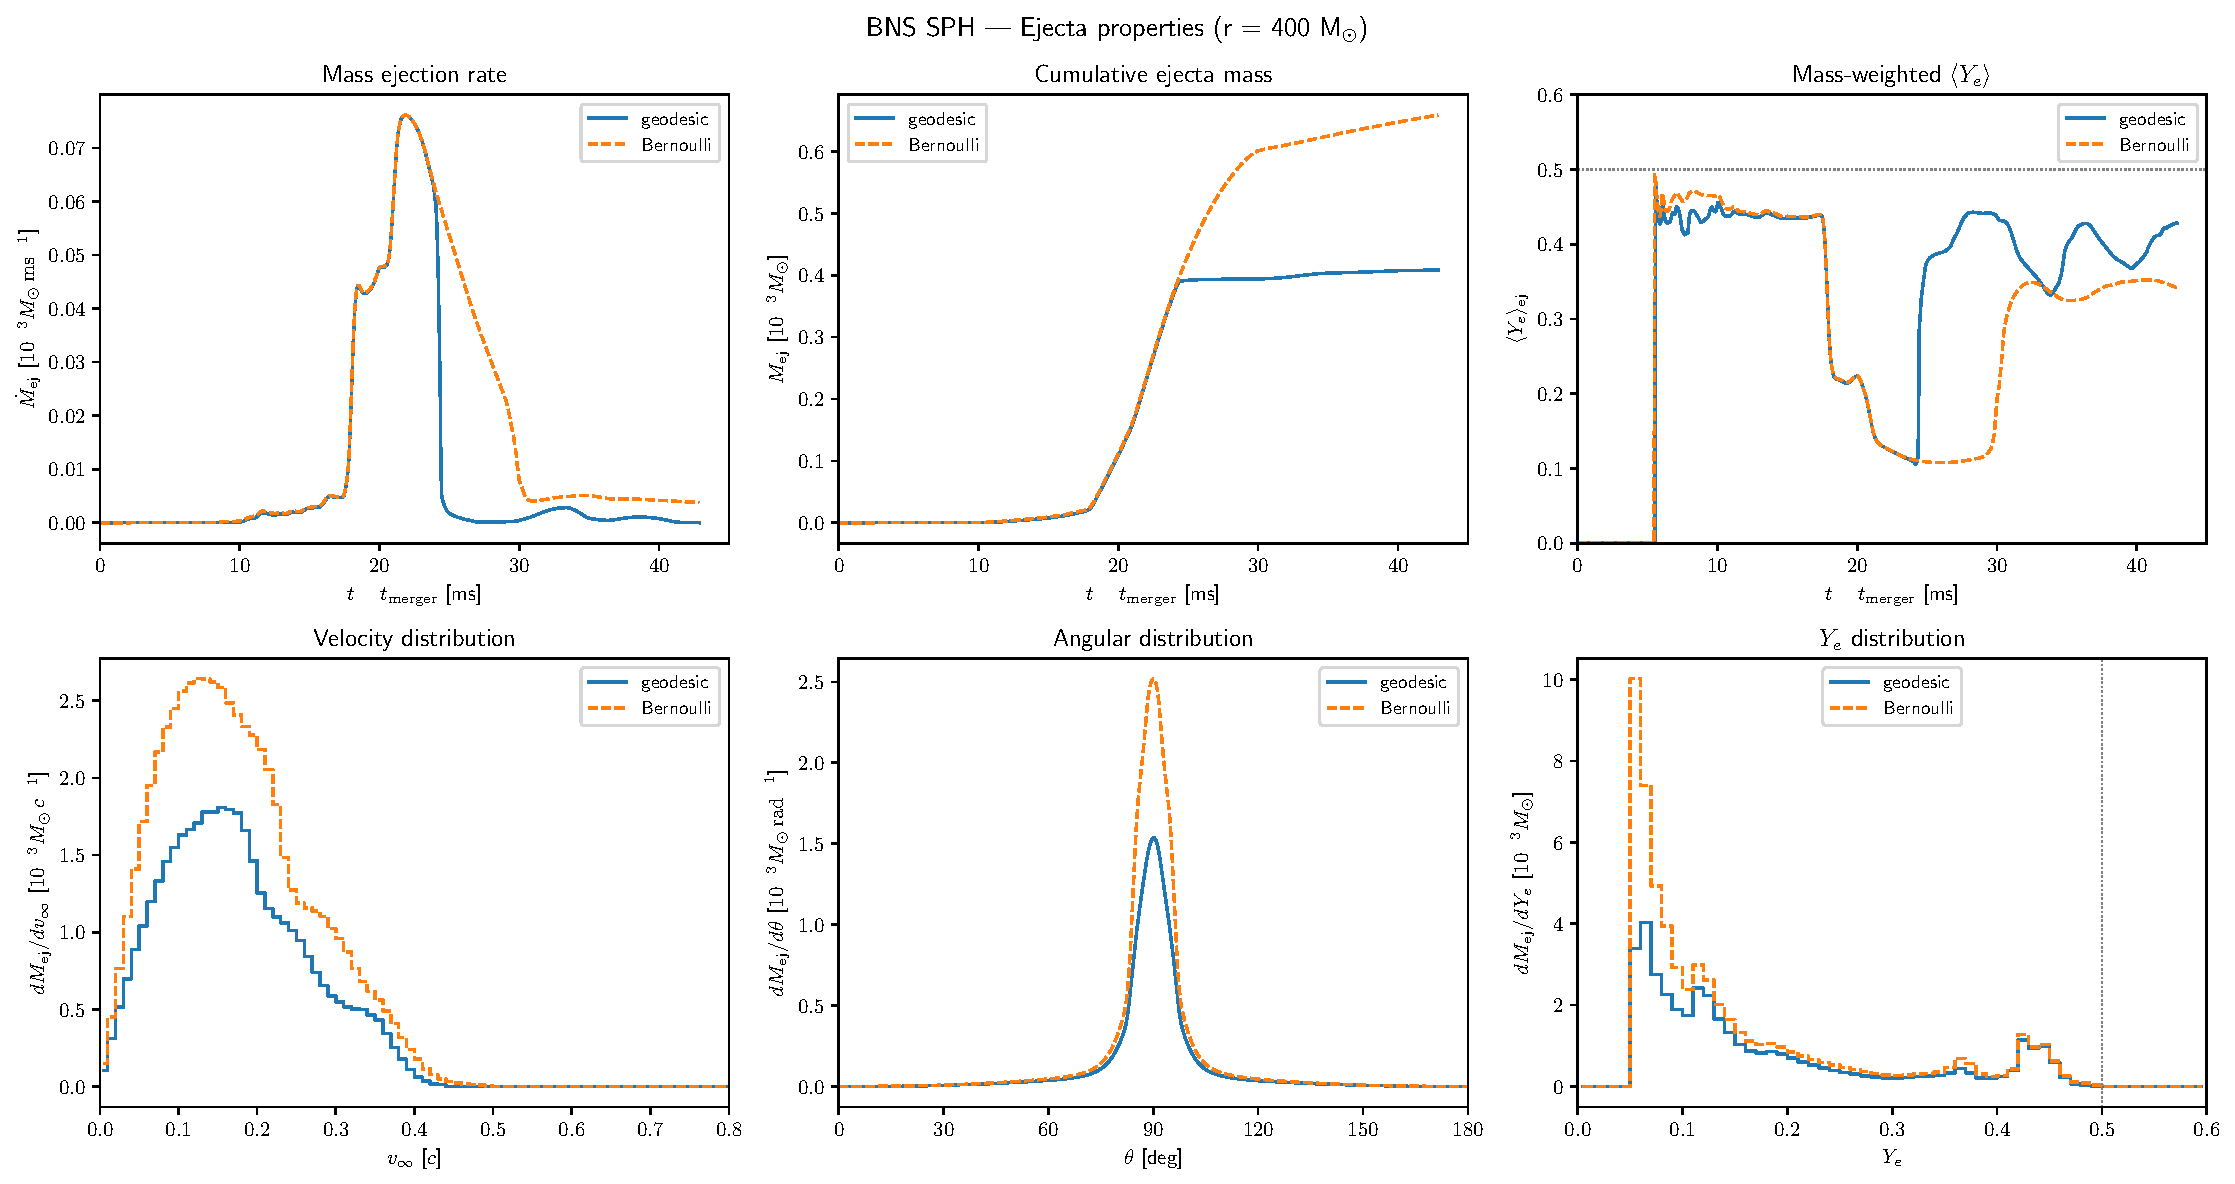
\includegraphics[width=1.0\textwidth]{Figures/fig_ejecta.pdf}
  \caption{Example of the ejecta analysis described above.}
  \label{Fig:fig_ejecta}
\end{figure}

\subsection*{Neutrino analysis}
\subsubsection*{Spherical output}
The neutrino analysis likewise operates on data dumped onto AthenaK spheres, with
one output block per variable:
\begin{verbatim}
<output2>
file_type = sph
variable  = rad_m1_N
dt        = 10.0
radius    = 400.0
ntheta    = 256
\end{verbatim}
Eight variables are required at each output time and radius: the Eulerian
energy-flux covector per species $F_i$ (\var{rad\_m1\_F}), the Eulerian energy
density per species $E$ (\var{rad\_m1\_E}), the number density per species $N$
(\var{rad\_m1\_N}), the ADM three-metric $\gamma_{ij}$ (\var{adm}), the lapse
$\alpha$ (\var{z4c\_alpha}) and the three shift components $\beta^i$
(\var{z4c\_betax}, \var{z4c\_betay}, \var{z4c\_betaz}). Useful radii are again
$300.0$ and $400.0$, and the same trade-off applies when choosing \var{dt}.

\subsubsection*{Pipeline}
The pipeline lives in the same \var{kplot.sphere} subpackage, where the
\var{neutrinos} module, exposed as the console script \var{kplot-sphere-neutrinos},
does the bulk of the computation. As input it takes the batchtools segment
directories containing the sph output (\var{-{}-sph-dir}), the extraction radius
(\var{-{}-radius}), the job name (\var{-{}-jobname}) and the output directory
(\var{-{}-output-dir}); no EOS table is needed here. As for the ejecta, all of them can
be left to \var{run\_analysis.sh}, which sets them from \var{config.ini} and can also
produce the plots.

\subsubsection*{Workflow}
The supported species are $\nu_e$ (\var{nue}), $\bar{\nu}_e$ (\var{nua}), $\nu_x$
(\var{nux}) and $\bar{\nu}_x$ (\var{anux}), where $\nu_x$ stands for the
heavy-lepton neutrinos; they follow AthenaK's M1 species ordering $s=0\dots3$.

\step{File matching} The pipeline first indexes the \var{rad\_m1\_F} files and
builds a time list for the \var{adm} and gauge files by reading only their VTK
header. This is necessary because the M1 and the metric output may use different
counter series (e.g.\ after a restart) even though they cover the same simulation
times. Taking the times of the neutrino fluxes $F$ as the baseline, the nearest
\var{adm}, \var{z4c\_alpha} and \var{z4c\_beta*} file in time is selected for each
snapshot; snapshots without a match inside the tolerance are skipped and reported.
The data are then loaded with the \var{SphericalData} class of plot-tools
(\url{https://github.com/jfields7/plot-tools}), and separate workers process each
snapshot to compute the neutrino luminosities and average energies.

\step{Angular weights and duplicates} From the flux file we take the time, the
radius $r$, the angles $\theta$, $\phi$, and the native AthenaK surface weights
$w=r^2 d\Omega$ (Gauss--Legendre in $\mu=\cos\theta$, uniform in $\phi$), which are
used directly for the surface integrals. The $\theta$ bin edges for the angular
diagnostics are built from the first snapshot. As in the ejecta analysis, the
duplication correction is derived from \var{z4c\_alpha} and applied to all eight
output variables.

\step{Radial projection} For each species we extract the flux components $F_x$,
$F_y$, $F_z$, the energy density $E$ and the number density $N$, and raise the index
on the flux with the inverse three-metric:
\begin{align}
  F^x &= \gamma^{xx}F_x+\gamma^{xy}F_y+\gamma^{xz}F_z\\
  F^y &= \gamma^{xy}F_x+\gamma^{yy}F_y+\gamma^{yz}F_z\\
  F^z &= \gamma^{xz}F_x+\gamma^{yz}F_y+\gamma^{zz}F_z
\end{align}
The inverse three-metric is computed component-wise from the determinant $\gamma$:
\begin{align}
  \gamma &= g_{xx}g_{yy}g_{zz}+2g_{xy}g_{xz}g_{yz}-g_{xx}g_{yz}^2-g_{yy}g_{xz}^2-g_{zz}g_{xy}^2\\
  \gamma^{xx} &= \left(g_{yy}g_{zz}-g_{yz}^2\right)/\gamma\\
  \gamma^{yy} &= \left(g_{xx}g_{zz}-g_{xz}^2\right)/\gamma\\
  \gamma^{zz} &= \left(g_{xx}g_{yy}-g_{xy}^2\right)/\gamma\\
  \gamma^{xy} &= \left(g_{xz}g_{yz}-g_{xy}g_{zz}\right)/\gamma\\
  \gamma^{xz} &= \left(g_{xy}g_{yz}-g_{xz}g_{yy}\right)/\gamma\\
  \gamma^{yz} &= \left(g_{xy}g_{xz}-g_{yz}g_{xx}\right)/\gamma
\end{align}
Following THC, the radial direction is normalized with the spatial block of the
inverse four-metric, $g^{ij}_4=\gamma^{ij}-\beta^i\beta^j/\alpha^2$:
\begin{align}
  g^{xx}_4&=\gamma^{xx}-\beta^x\beta^x / \alpha^2 &
  g^{xy}_4&=\gamma^{xy}-\beta^x\beta^y / \alpha^2\\
  g^{yy}_4&=\gamma^{yy}-\beta^y\beta^y / \alpha^2 &
  g^{xz}_4&=\gamma^{xz}-\beta^x\beta^z / \alpha^2\\
  g^{zz}_4&=\gamma^{zz}-\beta^z\beta^z / \alpha^2 &
  g^{yz}_4&=\gamma^{yz}-\beta^y\beta^z / \alpha^2
\end{align}
The radial vector is constructed from the angles $(\theta,\phi)$ and the radius of
the sphere,
\begin{align}
  r_x &= r\sin{\theta}\cos{\phi}, &
  r_y &= r\sin{\theta}\sin{\phi}, &
  r_z &= r\cos{\theta},
\end{align}
and its metric-normalized magnitude is
\begin{align}
  |r|=\sqrt{g^{xx}_4r_x^2+g^{yy}_4r_y^2+g^{zz}_4r_z^2+2g^{xy}_4r_{x}r_{y}+2g^{xz}_4r_{x}r_{z}+2g^{yz}_4r_{y}r_{z}}.
\end{align}
The flux projected along the radial direction is then
\begin{align}
  F^r = \frac{r_{x}F^x+r_{y}F^y+r_{z}F^z}{|r|},
\end{align}
and the same projection applied to the shift gives
\begin{align}
  \beta^r = \frac{r_{x}\beta^{x}+r_{y}\beta^{y}+r_{z}\beta^{z}}{|r|}.
\end{align}

\step{Luminosity and average energy} The radial energy flux of each species is
\begin{align}
  F_{\mathrm{rad}}=\alpha F^r-\beta^r E .
\end{align}
Note that $E$ and $F_i$ are already densitized M1 variables, so no additional
$\sqrt{\gamma}$ enters the surface integral. The energy luminosity in code units is
\begin{align}
  L_{\mathrm{code}}=\sum F_{\mathrm{rad}}\,w ,
\end{align}
which is converted to erg\,s$^{-1}$ for each species. For the average energy we need
the number luminosity. The M1 number current $f_\nu^a$ is not part of the sph output,
so the number flux is reconstructed by assuming that the number and energy currents
are advected with the same radial velocity, $F^r_N \approx F_{\mathrm{rad}}\,N/E$
(exact in the free-streaming limit at the detector sphere). With $N$ converted from
fm$^{-3}$ to code units $M_\odot^{-3}$,
\begin{align}
  \dot{N}_{\mathrm{code}}=\sum \frac{F_{\mathrm{rad}}\,N_{\mathrm{code}}}{E}\,w ,
\end{align}
where the sum runs over the points with $E>0$. The flux-weighted average neutrino
energy per species is the ratio of the two,
\begin{align}
  \langle \epsilon_{\nu} \rangle = \frac{L_{\mathrm{code}}}{\dot{N}_{\mathrm{code}}},
\end{align}
converted to MeV. Finally, the angular distribution of the luminosity
$dL_\nu/d\theta$ is obtained by histogramming the outgoing part of the radial flux
($F_{\mathrm{rad}}>0$) in $\theta$ with weights $F_{\mathrm{rad}}w$ and dividing by
the bin width $\Delta\theta$.

\subsubsection*{Post-Processing}
The above workflow is applied to all spherical output snapshots and the results are
sorted in time. We store the energy luminosity $L_{\nu}$ and the average energy
$\langle \epsilon_{\nu} \rangle$ per species as time series, as well as the total
luminosity summed over all four species,
$L_{\mathrm{total}}=\sum_{\nu}L_{\nu}$. The angular profiles $dL_\nu/d\theta$ are
integrated over time with a midpoint Riemann sum and converted to erg, which gives
the time-integrated radiated energy per angle $dE_{\nu}/d\theta$ [erg\,rad$^{-1}$]
for each species. All of these are written to \var{.txt} files in \var{-{}-output-dir}
for easy processing: \var{Lnu\_E\_\{sp\}.txt}, \var{Lnu\_E\_total.txt},
\var{Eav\_\{sp\}.txt} and \var{dEnu\_dtheta\_\{sp\}.txt}. With the \var{-{}-plot} flag
of \var{run\_analysis.sh} one can plot the neutrino luminosity and the average
neutrino energy for each species; the results look like Fig.~\ref{Fig:fig_neutrino}.
\begin{figure}[t]
  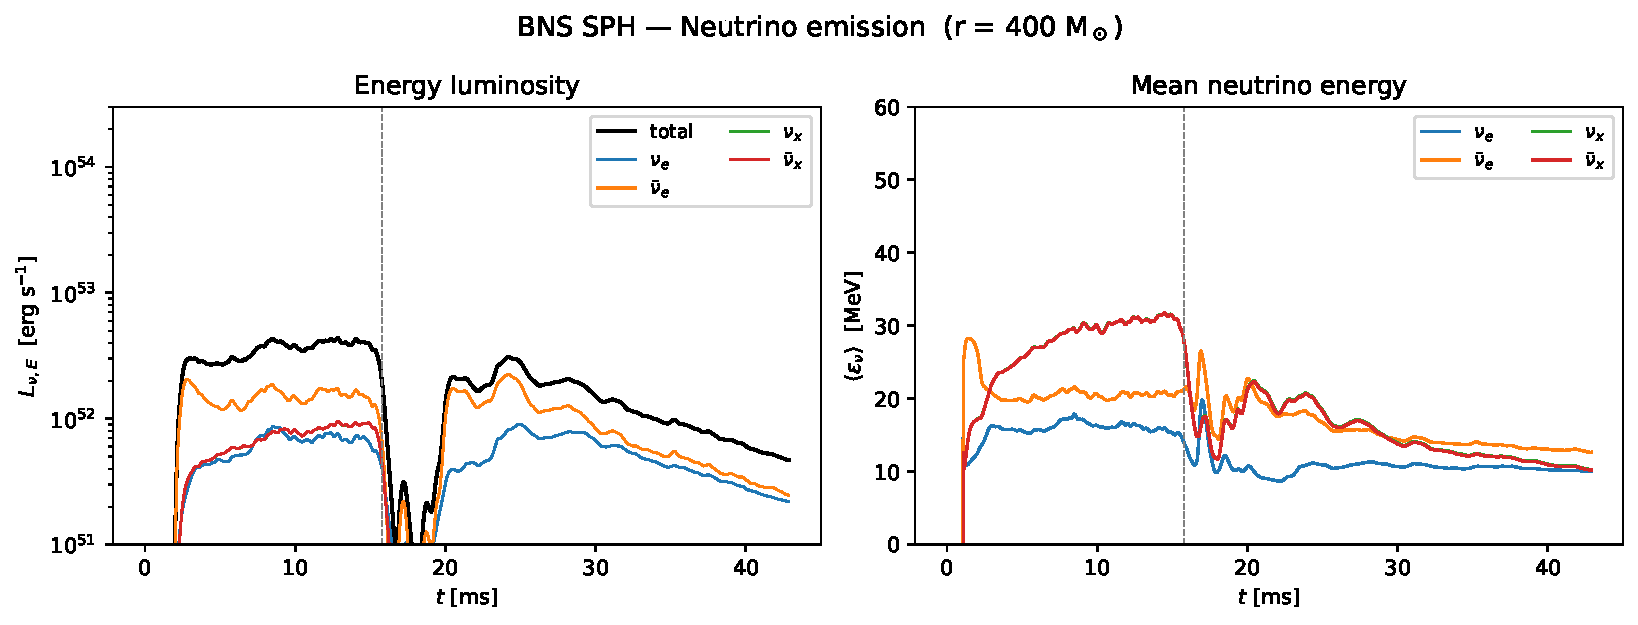
\includegraphics[width=\textwidth]{Figures/fig_neutrino.pdf}
  \caption{Example of the neutrino analysis described above.}
  \label{Fig:fig_neutrino}
\end{figure}

\end{document}
